\documentclass{article}

\usepackage[letterpaper]{geometry}
\usepackage{amsmath}
\usepackage{siunitx}
\usepackage{tikz}
\usepackage{gnuplot-lua-tikz}
\usepackage{minted}

\usemintedstyle{autumn}

\title{4125 HW 8}
\author{Duncan Wilkie}
\date{9 May 2022}

\begin{document}

\maketitle

\section*{7.20}
The quantum volume at this temperature is
\[
  v_{Q}=\left( \frac{h}{\sqrt{2\pi m_{e}kT}} \right)^{3}
  =\left( \frac{\SI{6.67e-34}{J\cdot s}}{\sqrt{2\pi (\SI{9.11e-31}{kg})(\SI{1.38e-23}{J/K})(\SI{e7}{K})}} \right)^{3}
  =\SI{1.34e-32}{m^{3}}
\]
Therefore, the volume per electron (the reciprocal of the density of the electrons) is on the order of the quantum volume,
so neither the condition for Boltzmann statistics ($V/N\gg v_{Q}$) or that for a Fermi gas ($V/N\ll v_{Q}$) are satisfied.

\section*{7.39}
The change of variables $\epsilon=hc/\lambda$, $d\epsilon=-\frac{hc}{\lambda^{2}}d\lambda$ results in
\[
  \frac{U}{V}=\int_{\infty}^{0}\frac{8\pi(hc/\lambda)^{3}/(hc)^{3}}{e^{hc/\lambda kT}-1}\left( -\frac{hc}{\lambda^{2}}d\lambda \right)
  =\int_{0}^{\infty}\frac{8\pi hc/\lambda^{5}}{e^{hc/\lambda kT}-1}d\lambda
\]
The spectrum is then
\[
  u(\lambda)=\frac{8\pi hc/\lambda^{5}}{e^{hc/\lambda kT}-1}
\]
which can be plotted as
\begin{center}
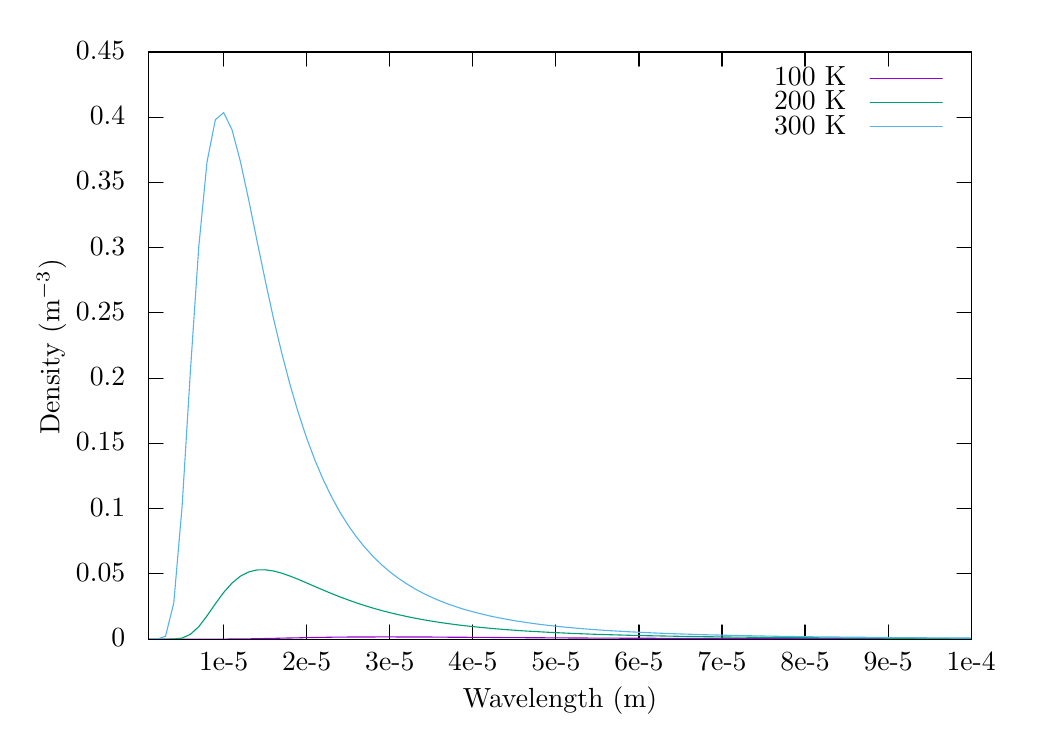
\begin{tikzpicture}[gnuplot]
%% generated with GNUPLOT 5.4p3 (Lua 5.3; terminal rev. Jun 2020, script rev. 115)
%% Fri 06 May 2022 07:46:54 PM CDT
\path (0.000,0.000) rectangle (12.500,8.750);
\gpcolor{color=gp lt color border}
\gpsetlinetype{gp lt border}
\gpsetdashtype{gp dt solid}
\gpsetlinewidth{1.00}
\draw[gp path] (1.504,0.985)--(1.684,0.985);
\draw[gp path] (11.947,0.985)--(11.767,0.985);
\node[gp node right] at (1.320,0.985) {$0$};
\draw[gp path] (1.504,1.813)--(1.684,1.813);
\draw[gp path] (11.947,1.813)--(11.767,1.813);
\node[gp node right] at (1.320,1.813) {$0.05$};
\draw[gp path] (1.504,2.642)--(1.684,2.642);
\draw[gp path] (11.947,2.642)--(11.767,2.642);
\node[gp node right] at (1.320,2.642) {$0.1$};
\draw[gp path] (1.504,3.470)--(1.684,3.470);
\draw[gp path] (11.947,3.470)--(11.767,3.470);
\node[gp node right] at (1.320,3.470) {$0.15$};
\draw[gp path] (1.504,4.299)--(1.684,4.299);
\draw[gp path] (11.947,4.299)--(11.767,4.299);
\node[gp node right] at (1.320,4.299) {$0.2$};
\draw[gp path] (1.504,5.127)--(1.684,5.127);
\draw[gp path] (11.947,5.127)--(11.767,5.127);
\node[gp node right] at (1.320,5.127) {$0.25$};
\draw[gp path] (1.504,5.956)--(1.684,5.956);
\draw[gp path] (11.947,5.956)--(11.767,5.956);
\node[gp node right] at (1.320,5.956) {$0.3$};
\draw[gp path] (1.504,6.784)--(1.684,6.784);
\draw[gp path] (11.947,6.784)--(11.767,6.784);
\node[gp node right] at (1.320,6.784) {$0.35$};
\draw[gp path] (1.504,7.613)--(1.684,7.613);
\draw[gp path] (11.947,7.613)--(11.767,7.613);
\node[gp node right] at (1.320,7.613) {$0.4$};
\draw[gp path] (1.504,8.441)--(1.684,8.441);
\draw[gp path] (11.947,8.441)--(11.767,8.441);
\node[gp node right] at (1.320,8.441) {$0.45$};
\draw[gp path] (2.453,0.985)--(2.453,1.165);
\draw[gp path] (2.453,8.441)--(2.453,8.261);
\node[gp node center] at (2.453,0.677) {1e-5};
\draw[gp path] (3.508,0.985)--(3.508,1.165);
\draw[gp path] (3.508,8.441)--(3.508,8.261);
\node[gp node center] at (3.508,0.677) {2e-5};
\draw[gp path] (4.563,0.985)--(4.563,1.165);
\draw[gp path] (4.563,8.441)--(4.563,8.261);
\node[gp node center] at (4.563,0.677) {3e-5};
\draw[gp path] (5.618,0.985)--(5.618,1.165);
\draw[gp path] (5.618,8.441)--(5.618,8.261);
\node[gp node center] at (5.618,0.677) {4e-5};
\draw[gp path] (6.673,0.985)--(6.673,1.165);
\draw[gp path] (6.673,8.441)--(6.673,8.261);
\node[gp node center] at (6.673,0.677) {5e-5};
\draw[gp path] (7.728,0.985)--(7.728,1.165);
\draw[gp path] (7.728,8.441)--(7.728,8.261);
\node[gp node center] at (7.728,0.677) {6e-5};
\draw[gp path] (8.782,0.985)--(8.782,1.165);
\draw[gp path] (8.782,8.441)--(8.782,8.261);
\node[gp node center] at (8.782,0.677) {7e-5};
\draw[gp path] (9.837,0.985)--(9.837,1.165);
\draw[gp path] (9.837,8.441)--(9.837,8.261);
\node[gp node center] at (9.837,0.677) {8e-5};
\draw[gp path] (10.892,0.985)--(10.892,1.165);
\draw[gp path] (10.892,8.441)--(10.892,8.261);
\node[gp node center] at (10.892,0.677) {9e-5};
\draw[gp path] (11.947,0.985)--(11.947,1.165);
\draw[gp path] (11.947,8.441)--(11.947,8.261);
\node[gp node center] at (11.947,0.677) {1e-4};
\draw[gp path] (1.504,8.441)--(1.504,0.985)--(11.947,0.985)--(11.947,8.441)--cycle;
\node[gp node center,rotate=-270] at (0.292,4.713) {Density ($\si{m^{-3}}$)};
\node[gp node center] at (6.725,0.215) {Wavelength ($\si{m}$)};
\node[gp node right] at (10.479,8.107) {100 K};
\gpcolor{rgb color={0.580,0.000,0.827}}
\draw[gp path] (10.663,8.107)--(11.579,8.107);
\draw[gp path] (1.504,0.985)--(1.609,0.985)--(1.715,0.985)--(1.820,0.985)--(1.926,0.985)%
  --(2.031,0.985)--(2.137,0.985)--(2.242,0.985)--(2.348,0.985)--(2.453,0.985)--(2.559,0.986)%
  --(2.664,0.987)--(2.770,0.988)--(2.875,0.990)--(2.981,0.992)--(3.086,0.994)--(3.192,0.997)%
  --(3.297,0.999)--(3.403,1.001)--(3.508,1.004)--(3.614,1.005)--(3.719,1.007)--(3.825,1.009)%
  --(3.930,1.010)--(4.036,1.011)--(4.141,1.012)--(4.247,1.012)--(4.352,1.012)--(4.458,1.013)%
  --(4.563,1.013)--(4.669,1.012)--(4.774,1.012)--(4.880,1.012)--(4.985,1.011)--(5.090,1.011)%
  --(5.196,1.010)--(5.301,1.009)--(5.407,1.009)--(5.512,1.008)--(5.618,1.007)--(5.723,1.007)%
  --(5.829,1.006)--(5.934,1.005)--(6.040,1.004)--(6.145,1.004)--(6.251,1.003)--(6.356,1.002)%
  --(6.462,1.002)--(6.567,1.001)--(6.673,1.001)--(6.778,1.000)--(6.884,0.999)--(6.989,0.999)%
  --(7.095,0.998)--(7.200,0.998)--(7.306,0.997)--(7.411,0.997)--(7.517,0.996)--(7.622,0.996)%
  --(7.728,0.995)--(7.833,0.995)--(7.939,0.995)--(8.044,0.994)--(8.150,0.994)--(8.255,0.994)%
  --(8.361,0.993)--(8.466,0.993)--(8.571,0.993)--(8.677,0.992)--(8.782,0.992)--(8.888,0.992)%
  --(8.993,0.992)--(9.099,0.991)--(9.204,0.991)--(9.310,0.991)--(9.415,0.991)--(9.521,0.991)%
  --(9.626,0.990)--(9.732,0.990)--(9.837,0.990)--(9.943,0.990)--(10.048,0.990)--(10.154,0.989)%
  --(10.259,0.989)--(10.365,0.989)--(10.470,0.989)--(10.576,0.989)--(10.681,0.989)--(10.787,0.989)%
  --(10.892,0.989)--(10.998,0.988)--(11.103,0.988)--(11.209,0.988)--(11.314,0.988)--(11.420,0.988)%
  --(11.525,0.988)--(11.631,0.988)--(11.736,0.988)--(11.842,0.988)--(11.947,0.988);
\gpcolor{color=gp lt color border}
\node[gp node right] at (10.479,7.799) {200 K};
\gpcolor{rgb color={0.000,0.620,0.451}}
\draw[gp path] (10.663,7.799)--(11.579,7.799);
\draw[gp path] (1.504,0.985)--(1.609,0.985)--(1.715,0.985)--(1.820,0.986)--(1.926,0.998)%
  --(2.031,1.046)--(2.137,1.142)--(2.242,1.280)--(2.348,1.433)--(2.453,1.577)--(2.559,1.696)%
  --(2.664,1.783)--(2.770,1.837)--(2.875,1.863)--(2.981,1.865)--(3.086,1.850)--(3.192,1.822)%
  --(3.297,1.785)--(3.403,1.743)--(3.508,1.698)--(3.614,1.652)--(3.719,1.607)--(3.825,1.563)%
  --(3.930,1.521)--(4.036,1.482)--(4.141,1.445)--(4.247,1.410)--(4.352,1.378)--(4.458,1.348)%
  --(4.563,1.321)--(4.669,1.296)--(4.774,1.273)--(4.880,1.251)--(4.985,1.232)--(5.090,1.214)%
  --(5.196,1.197)--(5.301,1.182)--(5.407,1.168)--(5.512,1.155)--(5.618,1.144)--(5.723,1.133)%
  --(5.829,1.123)--(5.934,1.114)--(6.040,1.105)--(6.145,1.098)--(6.251,1.090)--(6.356,1.084)%
  --(6.462,1.078)--(6.567,1.072)--(6.673,1.067)--(6.778,1.062)--(6.884,1.057)--(6.989,1.053)%
  --(7.095,1.049)--(7.200,1.045)--(7.306,1.042)--(7.411,1.039)--(7.517,1.036)--(7.622,1.033)%
  --(7.728,1.031)--(7.833,1.028)--(7.939,1.026)--(8.044,1.024)--(8.150,1.022)--(8.255,1.020)%
  --(8.361,1.018)--(8.466,1.017)--(8.571,1.015)--(8.677,1.014)--(8.782,1.012)--(8.888,1.011)%
  --(8.993,1.010)--(9.099,1.009)--(9.204,1.008)--(9.310,1.007)--(9.415,1.006)--(9.521,1.005)%
  --(9.626,1.004)--(9.732,1.003)--(9.837,1.002)--(9.943,1.002)--(10.048,1.001)--(10.154,1.000)%
  --(10.259,1.000)--(10.365,0.999)--(10.470,0.998)--(10.576,0.998)--(10.681,0.997)--(10.787,0.997)%
  --(10.892,0.996)--(10.998,0.996)--(11.103,0.996)--(11.209,0.995)--(11.314,0.995)--(11.420,0.994)%
  --(11.525,0.994)--(11.631,0.994)--(11.736,0.993)--(11.842,0.993)--(11.947,0.993);
\gpcolor{color=gp lt color border}
\node[gp node right] at (10.479,7.491) {300 K};
\gpcolor{rgb color={0.337,0.706,0.914}}
\draw[gp path] (10.663,7.491)--(11.579,7.491);
\draw[gp path] (1.504,0.985)--(1.609,0.985)--(1.715,1.020)--(1.820,1.445)--(1.926,2.675)%
  --(2.031,4.387)--(2.137,5.963)--(2.242,7.045)--(2.348,7.581)--(2.453,7.671)--(2.559,7.456)%
  --(2.664,7.058)--(2.770,6.570)--(2.875,6.052)--(2.981,5.541)--(3.086,5.058)--(3.192,4.614)%
  --(3.297,4.213)--(3.403,3.854)--(3.508,3.536)--(3.614,3.254)--(3.719,3.007)--(3.825,2.789)%
  --(3.930,2.597)--(4.036,2.428)--(4.141,2.280)--(4.247,2.149)--(4.352,2.033)--(4.458,1.931)%
  --(4.563,1.840)--(4.669,1.760)--(4.774,1.689)--(4.880,1.625)--(4.985,1.568)--(5.090,1.518)%
  --(5.196,1.472)--(5.301,1.431)--(5.407,1.395)--(5.512,1.361)--(5.618,1.332)--(5.723,1.305)%
  --(5.829,1.280)--(5.934,1.258)--(6.040,1.238)--(6.145,1.219)--(6.251,1.203)--(6.356,1.187)%
  --(6.462,1.173)--(6.567,1.160)--(6.673,1.149)--(6.778,1.138)--(6.884,1.128)--(6.989,1.119)%
  --(7.095,1.110)--(7.200,1.103)--(7.306,1.095)--(7.411,1.089)--(7.517,1.083)--(7.622,1.077)%
  --(7.728,1.072)--(7.833,1.067)--(7.939,1.062)--(8.044,1.058)--(8.150,1.054)--(8.255,1.050)%
  --(8.361,1.047)--(8.466,1.043)--(8.571,1.040)--(8.677,1.038)--(8.782,1.035)--(8.888,1.032)%
  --(8.993,1.030)--(9.099,1.028)--(9.204,1.026)--(9.310,1.024)--(9.415,1.022)--(9.521,1.020)%
  --(9.626,1.019)--(9.732,1.017)--(9.837,1.016)--(9.943,1.014)--(10.048,1.013)--(10.154,1.012)%
  --(10.259,1.011)--(10.365,1.010)--(10.470,1.008)--(10.576,1.008)--(10.681,1.007)--(10.787,1.006)%
  --(10.892,1.005)--(10.998,1.004)--(11.103,1.003)--(11.209,1.003)--(11.314,1.002)--(11.420,1.001)%
  --(11.525,1.001)--(11.631,1.000)--(11.736,0.999)--(11.842,0.999)--(11.947,0.998);
\gpcolor{color=gp lt color border}
\draw[gp path] (1.504,8.441)--(1.504,0.985)--(11.947,0.985)--(11.947,8.441)--cycle;
%% coordinates of the plot area
\gpdefrectangularnode{gp plot 1}{\pgfpoint{1.504cm}{0.985cm}}{\pgfpoint{11.947cm}{8.441cm}}
\end{tikzpicture}

%%% Local Variables:
%%% mode: latex
%%% TeX-master: "gnuplot-lua-tikz.sty"
%%% End:

\end{center}
The spectrum is a constant multiple of the function $\frac{1/x^{5}}{e^{1/x}-1}$ where $x=\lambda kT/hc$; we can minimize this numerically.
For fun, we can implement the numerical algorithm in Scheme, as below:
\begin{minted}{scheme}
(define (u x)
(/ (/ (expt x 5))
   (- (exp (/ x))
      1)))

(define (cdiff f x h)
  (/ (- (f (+ x (/ h 2)))
	(f (- x (/ h 2))))
     h))

(define (sign x)
  (if (negative? x)
      -1
      1))

(define (bisect f interval tol)
  (let*
      ((mid (/ (+ (cadr interval) (car interval)) 2))
       (fmid (f mid)))
    (if (< (abs fmid) tol)
	(list mid fmid)
	(bisect f
		(if
		 (= (sign fmid) (sign (f (cadr interval))))
		 (list (car interval) mid)
		 (list mid (cadr interval)))
		tol))))

(bisect (lambda (x) (cdiff u x 0.001))
	'(0.1 1)
	0.00001)
\end{minted}
Evaluating this in the Guile REPL, \newline
\verb|=> (0.20140608847141267 -7.53436424361098e-6)| \newline
so the maximum occurs at
\[
  \lambda kT/hc=0.20141
  \Leftrightarrow \lambda=\frac{hc}{(4.965)kT}
\]
This lower than the peak in the energy spectrum because lower wavelengths have disproportionately large amounts of associated energy
due to the nonlinear dependence of the two quantities on each other; therefore, the wavelength distribution skews more leftward.

\section*{7.44a}
The Planck distribution is the occupancy for this system; the sum over all possible energy states is the total number of particles.
Each mode has two possible photons corresponding to it, due to opposite polarizations.
We then can write, using $n$ to denote the magnitude of the vector $(n_{x},n_{y},n_{z})$
\[
  N=2\sum_{n_{x}}\sum_{n_{y}}\sum_{n_{z}}\overline{n}_{Pl}(\epsilon)
  =\sum_{n_{x},n_{y},n_{z}}\frac{2}{e^{hcn/2LkT}-1}
\]
Writing the sums as an integral in spherical coordinates over an $n$-space octant,
\[
  N=\int_{0}^{\infty}\int_{0}^{\pi/2}\int_{0}^{\pi/2}n^{2}\sin\theta\frac{2}{e^{hcn/2LkT}-1}dnd\phi d\theta
\]
The angular integrals evaluate to $\pi/2$, and we can make the change of variables to $x=hcn/2LkT$
(in which case $n=2LkTx/hc$ and $dn=2LkTdx/hc$) to obtain
\[
  N=\frac{\pi}{2}\int_{\infty}^{0}\left( \frac{2LkT}{hc}x \right)^{2}\frac{2}{e^x-1}\left(  -\frac{2LkT}{hc}\right)dx
  =\pi\left( \frac{2LkT}{hc}\right)^{3}\int_{0}^{\infty}\frac{x^{2}}{e^{x}-1}dx
\]
Identifying $L^{3}=V$,
\[
  N=8\pi V\left( \frac{kT}{hc} \right)^{3}\int_{0}^{\infty}\frac{x^{2}}{e^{x}-1}dx
\]
\newpage
We can add to our growing Scheme numerical methods library:
\begin{minted}{scheme}
(use-modules (srfi srfi-1)
	     (srfi srfi-8))

(define (f x)
  (/ (expt x 2)
     (- (exp x) 1)))

(define (simpstep f a b)
  (* (/ (- b a) 6)
     (+ (f a)
	(f b)
	(* 4 (f (/ (+ a b) 2))))))

(define (simpson f a b n)
  (let ((step (/ (- b a) n)))
    (receive (as bs)
	     (unzip2 (unfold (lambda (x) (>= x b))
			     (lambda (x) (list x (+ x step)))
			     (lambda (x) (+ x step))
			     a))
      (fold + 0 (map (lambda (x y) (simpstep f x y))
		     as
		     bs)))))

(simpson f 1e-10 100 1200000)
\end{minted}
This evaluates (impressively quickly, for a single-threaded interpreted language) to \newline
\verb|=> 2.404113806317145| \newline
so we may write
\[
  N=8\pi V\left( \frac{kT}{hc} \right)^{3}(2.4041)
\]

\section*{7.44c}
Plugging these values into our formula,
\[
  N=8\pi(\SI{1}{m})\left( \frac{(\SI{1.38e-23}{J/K})(\SI{300}{K})}{(\SI{6.67e-34}{J\cdot s})(\SI{3e8}{m/s})} \right)^{3}(2.4041)
  =\SI{5.24e14}{photons}
\]
\[
  N=8\pi(\SI{1}{m})\left( \frac{(\SI{1.38e-23}{J/K})(\SI{1500}{K})}{(\SI{6.67e-34}{J\cdot s})(\SI{3e8}{m/s})} \right)^{3}(2.4041)
  =\SI{6.69e16}{photons}
\]
\[
  N=8\pi(\SI{1}{m})\left( \frac{(\SI{1.38e-23}{J/K})(\SI{2.73}{K})}{(\SI{6.67e-34}{J\cdot s})(\SI{3e8}{m/s})} \right)^{3}(2.4041)
  =\SI{4.03e8}{photons}
\]

\section*{7.53a}
The peak of the blackbody wavelength spectrum was derived in problem 7.39 to be at
\[
  \lambda = \frac{hc}{(4.965)kT}=\frac{16\pi^{2}GM}{(4.965)c^{2}}=\frac{16\pi^{2}(\SI{6.67e-11}{Nm^{2}/kg^{2}})(\SI{2e30}{kg})}
  {(4.965)(\SI{3e8})^{2}}
\]
\[
  =\SI{47.1}{km}
\]
Equating the expression for the surface area to $4\pi R^{2}$, the radius is
\[
  R=\frac{2GM}{c^{2}}=\frac{2(\SI{6.67e-11}{Nm^{2}/kg^{2}})(\SI{2e30}{kg})}{(\SI{3e8}{m/s})^{2}}
  =\SI{2.96}{km}
\]
The radiated wavelength is predicted to be significantly larger than the black hole itself.

\section*{7.53b}
Taking the black hole to be a perfect blackbody, the total power radiated is
\[
  P=\sigma AT^{4}=\frac{2\pi^{5}k^{4}}{15h^{3}c^{2}}\left( \frac{16\pi G^{2}M^{2}}{c^{4}} \right)
  \left( \frac{hc^{3}}{16\pi^{2}kGM} \right)^{4}
  =\frac{hc^{6}}{15\cdot 8\cdot16^{2}\pi^{6}G^{2}M^{2}}
\]
\[
  \frac{(\SI{6.63e-34}{J\cdot s})(\SI{3e8}{m/s})^{6}}
  {15\cdot 8\cdot16^{2}\pi^{6}(\SI{6.67e-11}{Nm^{2}/kg^{2}})^{2}(\SI{2e30}{kg})^{2}}
  =\SI{9.20e-31}{W}
\]

\section*{7.53c}
The rate of change of the energy of the black hole is the negative of the power expression above, i.e.
\[
  \frac{d}{dt}(Mc^{2})=-\frac{hc^{6}}{15\cdot 8\cdot 16^{2}\pi^{6}G^{2}M^{2}}
\]
Separating the variables,
\[
  M^{2}{dM}=-\frac{hc^{4}}{15\cdot 8\cdot 16^{2}\pi^{6}G^{2}}dt
\]
Integrating and applying the initial condition $M(0)=M_{0}$,
\[
  \frac{M^{3}}{3}=\frac{M_{0}^{3}}{3}-\frac{hc^{4}}{15\cdot 8\cdot 16^{2}\pi^{6}G^{2}}t
\]
\[
  \Leftrightarrow M(t)=\sqrt[3]{M_{0}^{3}-\frac{hc^{4}}{40\cdot16^{2}\pi^{6}G^{2}}t}
\]
This is equal to zero when
\[
  \frac{hc^{4}}{40\cdot 16^{2}\pi^{6}G^{2}}t_{l}=M_{0}^{3}
  \Leftrightarrow t_{l}=\frac{40\cdot 16^{2}\pi^{6}G^{2}M_{0}^{3}}{hc^{4}}
\]

\section*{7.53d}
Evaluating the last equation above at $M_{0}$ equal to one solar mass,
\[
  t_{l}=\frac{40\cdot 16^{2}\pi^{6}(\SI{6.67e-11}{Nm^{2}/kg^{2}})^{2}(\SI{2e30}{kg})^{3}}{(\SI{6.63e-34}{J s})(\SI{3e8}{m/s})^{4}}
  =\SI{6.51e76}{s}=\SI{2.07e69}{yr}
\]
\[
  \approx\textrm{2 Morbillion years}
\]
This is longer than the age of the universe by 60 orders of magnitude.

\section*{7.53e}
This can be written
\[
  M_{0}=\sqrt[3]{\frac{hc^{4}}{40\cdot 16^{2}\pi^{6}G^{2}}t_{l}}
  =\sqrt[3]{\frac{(\SI{6.63e-34}{Js})(\SI{3e8}{m/s})^{4}}{40\cdot 16^{2}\pi^{6}(\SI{6.67e-11}{Nm^{2}/kg^{2}})^{2}}(10^{10})}
  =\SI{10.7e7}{kg}
\]
Doing the same peak wavelength calculation as before,
\[
  \lambda = \frac{16\pi^{2}GM}{(4.965)c^{2}}=\frac{16\pi^{2}(\SI{6.67e-11}{Nm^{2}/kg^{2}})(\SI{10.7e7}{kg})}{(4.965)(\SI{3e8})^{2}}
  =\SI{2.5e-18}{m}
\]
which corresponds to extremely high-energy gamma radiation.

\section{}
The magnitude of the momentum of an electron in the gas is
\[
  p=\sqrt{p_{x}^{2}+p_{y}^{2}}=\sqrt{\frac{h^{2}n_{x}^{2}}{4L^{2}}+\frac{h^{2}n_{y}^{2}}{4L^{2}}}=\frac{h}{2L}\sqrt{n_{x}^{2}+n_{y}^{2}}
  =\frac{hn}{2L}
\]
The total energy of the gas at $T=0$ is, proceeding similarly to the derivation for a nonrelativistic electron gas,
\[
  U=2\sum_{n_{x},n_{y}}\epsilon(\vec{n})=2\int_{0}^{n_{max}}\int_{0}^{\pi/2}\epsilon(n)n dnd\theta
\]
where the 2 accounts for the two distinct electronic spin states for each combination of $n_{x}$ and $n_{y}$,
the passage to integrals is justified by presuming the number of electrons, and we convert to polar coordinates in $n$ space.
We then apply the change of variables
\[
  \epsilon=\sqrt{p^{2}c^{2}+m^{2}c^{4}}=\sqrt{\frac{h^{2}n^{2}c^{2}}{4L^{2}}+m^{2}c^{4}}
  \Leftrightarrow n=\sqrt{\frac{4L^{2}}{h^{2}c^{2}}(\epsilon^{2}-m^{2}c^{4})}
\]
\[
  dn=\frac{4L^{2}\epsilon/h^{2}c^{2}}{\sqrt{\frac{4L^{2}}{h^{2}c^{2}}(\epsilon^{2}-m^{2}c^{4})}}d\epsilon
\]
to get
\[
  U={\pi}\int_{0}^{n_{max}}\epsilon(n)ndn=\int_{mc^{2}}^{\epsilon_{F}}\pi\epsilon\frac{4L^{2}\epsilon}{h^{2}c^{2}}d\epsilon
\]
implying the density of states (which is a probability distribution in the state energy variable whose expectation is the average energy of
the system) is the integrand
divided by $\epsilon$:
\[
  g(\epsilon) = \frac{4\pi L^{2}\epsilon}{h^{2}c^{2}}
\]

\section{}
Much like the nonrelativistic case, $\epsilon_{F}$ is the energy of an electron just on the surface of the circle in $n$ space, so
\[
  \epsilon_{F}=\sqrt{\frac{h^{2}n_{max}^{2}c^{2}}{4L^{2}}+m^{2}c^{4}}
\]
The total number of occupied states at $T=0$ is twice (due to spin) the volume of a quarter-circle with radius $n_{max}$ in $n$ space, i.e.
\[
  N=2\cdot{\frac{1}{4}}\pi n_{max}^{2}=\frac{\pi n_{max}^{2}}{2}
  \Leftrightarrow n_{max}=\sqrt{\frac{2N}{\pi}}
\]
Plugging this in to the formula for $\epsilon_{F}$,
\[
  \epsilon_{F}=\sqrt{\frac{Nh^{2}c^{2}}{2\pi L^{2}}+m^{2}c^{4}}
\]
In the nonrelativistic limit, the dominant contribution to the energy is the $m^{2}c^{4}$ term, i.e. $N/L^{2}$ is small in comparison.
Expanding using $\sqrt{a+x}\approx \sqrt{a}+\frac{x}{2a}$ when $x\to 0$,
\[
  \epsilon_{F}\approx mc^{2}+\frac{Nh^{2}c^{2}}{2\pi mc^{2}L^{2}}=mc^{2}+\frac{Nh^{2}}{2\pi mL^{2}}
\]
The first term is the rest mass of the electron at the Fermi surface, and the second term is precisely the nonrelativistic Fermi energy.
To see this, repeat the calculation above, but take $\epsilon_{F}=\frac{h^{2}n_{max}^{2}}{4mL^{2}}$ in accordance with the nonrelativistic
result $\epsilon(n)=\frac{p^{2}}{2m}=\frac{h^{2}n^{2}}{8mL^{2}}$.
\end{document}
%%% Local Variables:
%%% TeX-command-extra-options: "-shell-escape"
%%% mode: latex
%%% TeX-master: t
%%% End:
